\section{Diagrammes UML de Graphicus-02}

\begin{figure}[H]
    \centering
    \begin{tikzpicture}
        \begin{umlsystem}{Graphicus-02}
            \umlusecase[x=-2,y=5]{Activer une couche}
            \umlusecase[x=-2,y=3]{Cacher une couche}
            \umlusecase[y=1]{Ajouter une former sur la couche active}
            \umlusecase[y=-1]{Retirer une former sur la couche active}
            \umlusecase[x=4,y=4]{Changer l'état d'une couche}
        \end{umlsystem}

        \umlactor[y=2,x=-6]{Dessinateur}

        \umlassoc{Dessinateur}{usecase-1}
        \umlassoc{Dessinateur}{usecase-3}
        \umlassoc{Dessinateur}{usecase-2}
        \umlassoc{Dessinateur}{usecase-4}

        \umlinclude{usecase-1}{usecase-5}
        \umlinclude{usecase-2}{usecase-5}
        \umlextend{usecase-3}{usecase-4}
    \end{tikzpicture}
    \caption{Diagramme de cas d’utilisation UML de Graphicus-02}
\end{figure}

\begin{figure}[H]
    \centering
    \begin{tikzpicture}
        \umlstateinitial[name=init,x=-3,y=-1.5]
        \begin{umlstate}[name=main]{Couche créée}
            \umlbasicstate[name=0]{État initial}
            \umlbasicstate[name=1,x=4]{État actif}
            \umlbasicstate[name=2,x=4,y=-4]{État inactif}
            \umlbasicstate[name=3,y=-4]{État caché}

            \umltrans{0}{1}
            \umltrans{0}{2}
            \umltrans{0}{3}

            \umltrans{1}{2}
            \umltrans{1}{3}

            \umltrans{2}{1}
            \umltrans{2}{3}

            \umltrans{3}{1}
            \umltrans{3}{2}
        \end{umlstate}
        \umlstatefinal[x=7,y=-1.5, name=final]
        \umltrans{init}{main}
        \umltrans{main}{final}
    \end{tikzpicture}
    \caption{Diagramme d'états-transitions UML dee états d'une couche}
\end{figure}

\begin{figure}[H]
    \centering
    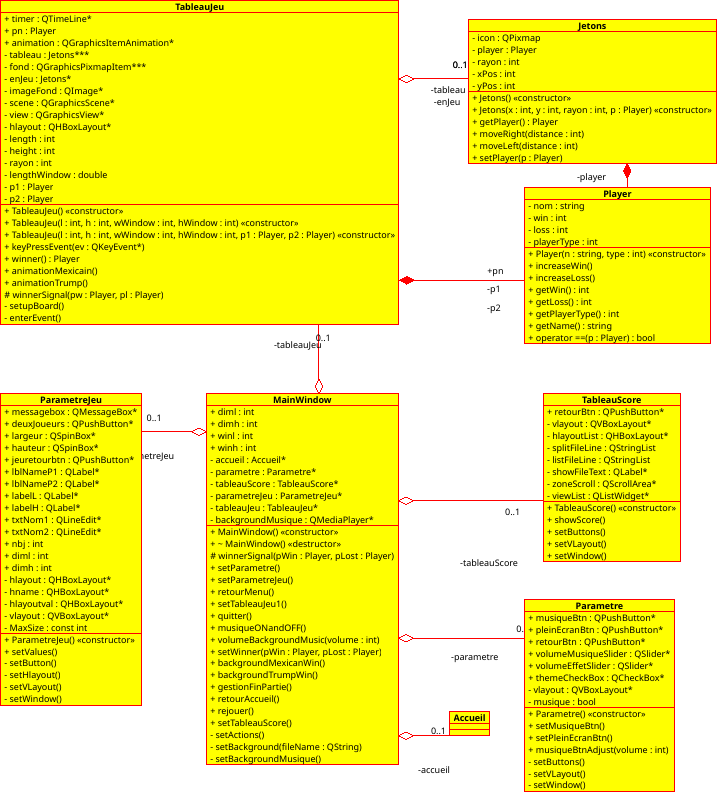
\includegraphics[width=6in]{img/classes}
    \caption{Diagramme de classes UML de Graphicus-02}
\end{figure}

\begin{figure}[H]
    \begin{tikzpicture}
        \begin{umlseqdiag}
            \umlactor[class=Utilisateur]{dessinateur}
            \umlobject[class=Canevas]{canevas}
            \umlobject[class=Couche]{couche}
            \umlobject[class=Vecteur]{vecteur}

            \begin{umlcall}[op={Canevas::ajoutFin()},return=bool]{dessinateur}{canevas}
                \begin{umlcall}[op={Couche::ajoutFin()},return=bool]{canevas}{couche}
                    \begin{umlcall}[op={Vecteur::ajoutFin()},return=bool]{couche}{vecteur}
                    \end{umlcall}
                \end{umlcall}
            \end{umlcall}
        \end{umlseqdiag}
    \end{tikzpicture}
    \caption{Diagramme de séquences UML de la fonction ajoutFin()}
\end{figure}

\section{Pseudocode de la fonction d’insertion de la classe vecteur}

\begin{algorithm}[H]
    \caption{Fonction d'insertion}
    \begin{algorithmic}[1]
        \Procedure{ajoutFin}{Forme *p\_forme}
        \If{capacite <= taille}
            \State doublerTaille()
        \EndIf
        \State Insérer la forme dans la dernière case du tableau
        \State Incrémenter taille
        \EndProcedure
    \end{algorithmic}
\end{algorithm}

\begin{algorithm}[H]
    \caption{Fonction qui double la taille}
    \begin{algorithmic}[1]
        \Procedure{doublerTaille}{}
        \State Créer un tableau deux fois plus grand
        \ForAll{forme dans le vecteur}
            \State Copier la forme de l'ancien tableau vers le nouveau tableau
        \EndFor
        \State Enregistrer l'adresse du nouveau tableau dans l'ancien tableau
        \EndProcedure
    \end{algorithmic}
\end{algorithm}

\section{Plan de tests de Graphicus-02}

Les tests sont entièrement automatisés.
Chaque test indique s'il est réussi ou s'il est en échec.
À la fin des tests, un résumé des tests s'affiche afin d'indiquer le nombre de tests réussis ainsi que le nombre de tests échoués.
Dans le cas où un ou des tests échouent, il suffit de consulter la sortie des tests pour trouver le ou les tests en échecs.
La description du test permet de cibler l'endroit approximatif d'une erreur.
Par ailleurs, malgré le fait que la classe \texttt{Tests} contient beaucoup de tests, certains extraits de plan de tests ont été reproduit dans le tableau suivant.

\begin{table}[H]
    \centering
    \caption{Exemple de plan de tests de la classe Rectangle}
    \begin{tabular}{p{2in}p{2in}p{2in}}
        \hline
        \bfseries Fonction & \bfseries Paramètre & \bfseries Résultat attendu\\
        \hline
        getLargeur & Rectangle() & 1\\
        getHauteur & Rectangle() & 1\\
        getAncrage & Rectangle() & \{0, 0\}\\
        aire & Rectangle() & 1\\
        \hline
        getLargeur & Rectangle(2, 3, \{4, 5\}) & 2\\
        getHauteur & Rectangle(2, 3, \{4, 5\}) & 3\\
        getAncrage & Rectangle(2, 3, \{4, 5\}) & \{4, 5\}\\
        aire & Rectangle(2, 3, \{4, 5\}) & 6\\
        \hline
        getLargeur & translater(2, 3) & 2\\
        getHauteur & translater(2, 3) & 3\\
        getAncrage & translater(2, 3) & \{6, 8\}\\
        aire & translater(2, 3) & 6\\
        \hline
        getLargeur & setAncrage({4, 5}) & 2\\
        getHauteur & setAncrage({4, 5}) & 3\\
        getAncrage & setAncrage({4, 5}) & \{4, 5\}\\
        aire & setAncrage({4, 5}) & 6\\
        \hline
    \end{tabular}
\end{table}
